
%(BEGIN_QUESTION)
% Copyright 2015, Tony R. Kuphaldt, released under the Creative Commons Attribution License (v 1.0)
% This means you may do almost anything with this work of mine, so long as you give me proper credit

Examine this partial schematic diagram for an overcurrent protection trip circuit, using a protective relay to perform the functions of instantaneous overcurrent (50) and/or time-overcurrent (51).  The electrical symbols inside each box reveal the components inside the circuit breaker and protective relay, respectively.  Screw heads are also shown as termination points for wires you will sketch between these devices to form a functional system.  Note that each of the relay's contacts will {\it close} when it commands the circuit breaker to trip, and that the auxiliary contacts inside the circuit breaker (52a and 52b) operate in unison with the high-current power contact (52):

$$\includegraphics[width=15.5cm]{i02861x01.eps}$$

First, sketch wires between the protective relay and the current transformer (CT) so that the CT's output current will drive the electromagnetic coils inside the protective relay, to actuate the trip contact(s) in the event of an overcurrent condition.

%\vskip 10pt

%Next, sketch wires between the protective relay and the circuit breaker so that the protective relay will energize the breaker's trip coil in the event of an {\it instantaneous overcurrent} condition only (i.e. a condition of extremely high line current through the power contacts of the circuit breaker).

%\vskip 10pt

%Next, sketch wires between the protective relay and the circuit breaker so that the protective relay will energize the breaker's trip coil in the event of a {\it time-overcurrent} condition only (i.e. a condition of mild overcurrent through the breaker's power contacts that persists longer than permissible for normal operation).

\vskip 10pt

Next, sketch wires between the protective relay and the circuit breaker so that the protective relay fulfills both the 50 ({\it instantaneous overcurrent}) function as well as the 51 ({\it time-overcurrent}) function.

\vskip 10pt

Finally, determine the effects of the following faults, and be prepared to explain why for each case:

\begin{itemize}
\item{} Fuse {\it blown} on 125 VDC station battery
\item{} Cable connecting CT to protective relay failed {\it shorted}
\item{} 52a breaker auxiliary switch contact failed {\it open}
\item{} 50 relay switch contact failed {\it open}
\item{} 51 relay switch contact failed {\it open}
\end{itemize}

\vskip 10pt

\underbar{file i02861}
%(END_QUESTION)





%(BEGIN_ANSWER)

No answers given here, but just a few hints.  The 52a and 52b auxiliary contacts within the circuit breaker serve to selectively disable the actuating coils, depending on the state of the breaker.  When the breaker is closed (i.e. power contact 52 conducting line current), contact 52a will be closed (permitting the trip coil to energize at the relay's command) and contact 52b will be open (prohibiting the close coil from energizing).  This should make sense: if the circuit breaker is already in the closed state, it would be pointless to allow the close coil to become energized and so the open 52b contact will prohibit that.
 
%(END_ANSWER)





%(BEGIN_NOTES)

\noindent
{\bf Trip circuit for 50 + 51 functions:}

$$\includegraphics[width=15.5cm]{i02861x02.eps}$$

%INDEX% Protective relay: instantaneous overcurrent (50)
%INDEX% Protective relay: time-overcurrent (51)

%(END_NOTES)


